In the following, the results of the conducted simulations are analyzed. The aim is to find an explanation for the transition between the presented growth regions of capillary rise. In particular, the transition from the linear region ($z(t)\sim t$) to the growth described by Lucas and Washburn ($z(t)\sim \sqrt{t}$) is considered. To account for potential influences by different contact angles, simulations were carried out with three different values. Additionally, simulations with activated non-equilibrium boundary conditions were conducted to analyze the influence of relaxation at the wall on capillary rise. Firstly, the equilibrium boundary condition is examined in Chapter \ref{sec: EquilibriumBoundaryCondition}, followed by a comparison with the non-equilibrium boundary condition in Section \ref{sec: outOfEquilibriumBoundaryCondition}.

\section{Preliminary Work}
During the course of this work, several simulations and investigations were conducted that were ultimately not pursued further or are included in this work. However, some of these works were essential to determine the simulation parameters. This includes simulations such as the examination of the \textit{mobility} or \textit{courant number} and different \textit{viscosity schemes}. Simulations with different discretizations of the computation domain, as well as the use of Adaptive Mesh Refinement (AMR), were also conducted. There were also simulations that did not directly contribute to determining the simulation parameters. These include simulations considering the \textit{pinning} effect, not mentioned in this work, or geometries that no longer correspond to those of this work but, despite simplifications, are closer to reality. These simulations are not considered further in this work.

Considering the dimensions used for the capillary and the liquids, it is expected that the influence of gravity is negligible. This could also be shown in separately conducted simulations. However, due to the low informative value of a comparison with simulations without gravity, it is not considered further. Thus, it becomes clear that one of the simplifications assumed by Lucas and Washburn does not apply in this case. A deviation from the prediction according to Equation \ref{eq: LW-Eq} can be attributed to the fact that a balance between capillary force and viscous drag is not sufficient to describe the capillary rise in early imbibition stages.

\section{Equilibrium Boundary Condition} 
\label{sec: EquilibriumBoundaryCondition}
The evaluation using only one of the employed contact angles is carried out in the following with an equilibrium contact angle of $\theta_{\mathrm{e}}=15^{\circ}$. A comparison of the simulation results for this contact angle with the Lucas-Washburn equation \ref{eq: LW-Eq} is shown in Figure \ref{fig: LW-PFF_comp}. The predicted imbibition length is depicted in red, and the simulation results are shown in black. To predict the same order of magnitude as the simulation, a correction factor had to be added to the Lucas-Washburn equation.
\todo{Adjust figure}
\begin{figure}[h]
    \centering
    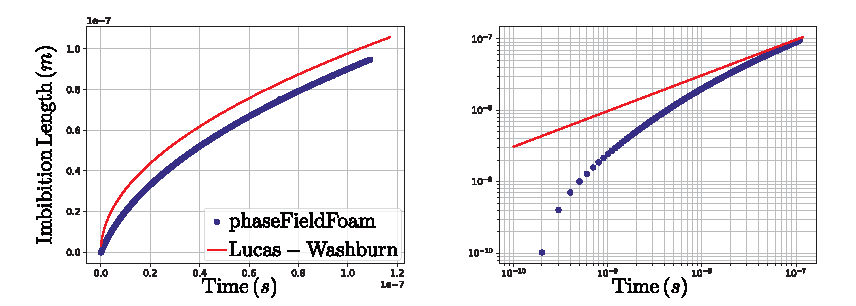
\includegraphics[width=.95\textwidth]{Pictures/LW-lin_loglog.pdf}
    \caption{Comparison of the growth predicted by Lucas-Washburn with the results from \texttt{phaseFieldFoam}}
    \label{fig: LW-PFF_comp}
\end{figure}
Figure \ref{fig: LW-PFF_comp} (a) provides a linear scaling, while \ref{fig: LW-PFF_comp} (b) uses a logarithmic scaling. The differences become even clearer in the logarithmic presentation. Initially, the slope of the simulation results is greater than that of the prediction until they finally converge. This indicates that the capillary rise initially follows the well-known Lucas-Washburn growth, as confirmed by many studies cited in Section \ref{sec: capillaryRise}.

To understand the differences in behavior, it is useful to consider the forces acting within the water column. Delanoy et al. \cite{delannoy2019DualRoleViscosity} attributed these differences to local dissipation. Hence, it is advisable to take a closer look at the area near the interface. Figure \ref{fig: eDiss_wedge} depicts the viscous forces in the water column near the contact line. This area is focused on as the forces in other parts of the water column are considerably lower. It is clear that the viscous forces are greatest near the contact line and directly at the wall. Two dissipative channels are formed. Here, the viscous forces near the contact line overlap with the viscous resistance caused by changes in the contact angle due to the system's dynamics. \todo{check!!!!}

\begin{figure}[h]
    \centering
    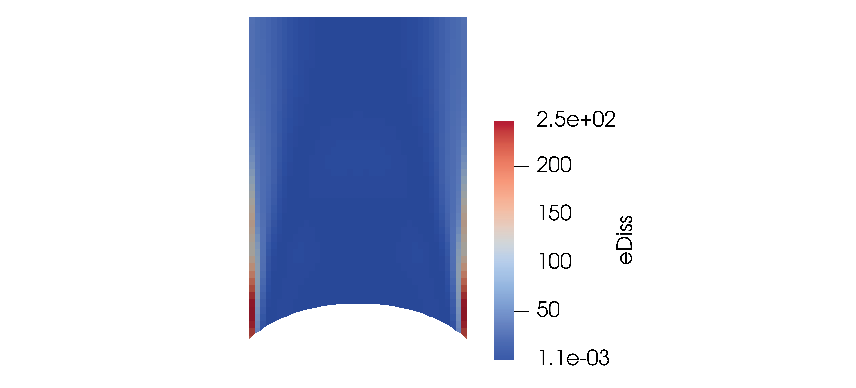
\includegraphics[width=.95\textwidth]{Pictures/eDiss_Wedge.pdf}
    \caption{Dissipative channels near the contact line.}
    \label{fig: eDiss_wedge}
\end{figure}

\begin{figure}[h]
    \centering
    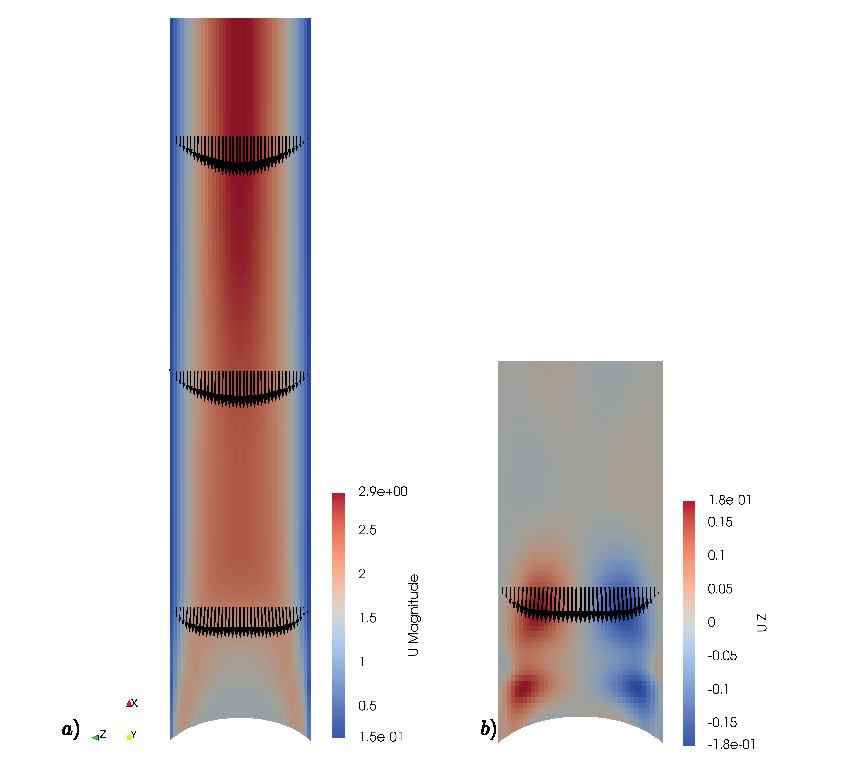
\includegraphics[width=.95\textwidth]{Pictures/Velo_Wedge.pdf}
    \caption{(a) Velocity field in the water column at $100ns$ and $\theta_{\mathrm{e}}=15^{\circ}$, (b) detailed view of recirculation near the interface.}
    \label{fig: Velofield_Wedge}
\end{figure}
Figure \ref{fig: Velofield_Wedge} visualizes the velocity field in the water and matches expectations. The water's velocity is highest in the center of the capillary (see (a)). To visualize the changing velocity field as it approaches the interface, vectors of the velocity field were also added for three levels. Far from the interface, the expected parabolic profile is observed. As one approaches the interface, it's evident how the flow in the center is decelerated, and a closer look at the vectors reveals that the flow is deflected to the edge. In (b), the section near the interface is enlarged, and instead of the magnitude of the velocity, only the component normal to the flow direction ($z$-direction) is visualized. It's clear that up to shortly before the flow, this component is negligible, and close to the interface, it increases significantly and seems to form two regions. One directly at the interface and close to the wall and another slightly further inside the water column. From the legend, it is clear that the order of magnitude compared to the velocity in the direction of flow differs by a decade. The area where the velocity change occurs is subsequently referred to as $\mathrm{W}$. Up to this area, it can be assumed that the flow corresponds to that described by Poiseuille and thus the viscous resistance corresponds to the Poiseuille viscous resistance. Thus, the viscous forces prevailing in $\mathrm{W}$ can be directly calculated from the simulation. The overall effective viscous forces are obtained from the simulation using Equation \ref*{eq: total_viscForce}, and the viscous resistance can be calculated with $F_{\eta}$ from Equation \ref*{eq: NewtonBalanceForcesOnly}. The difference between the two forces corresponds to the viscous forces prevailing in $\mathrm{W}$.

Furthermore, using the meniscus velocity, the theoretical Poiseuille viscous resistance and the resistance forces at the meniscus (Equation \todo{EQ}) are calculated. The equation described by Cox and Voinov (\ref*{eq: Cox-Voinov}) is used to predict the dynamic contact angle. It's often challenging to estimate the ratio of length scales since $l_{\mathrm{m}}$ usually assumes a length of $1nm$, and for $l$, several lengths, such as the radius, the length of the capillary, or even the length of $\mathrm{W}$, are assumed. In the following, a ratio of $l_{\mathrm{m}}/l\approx10$ is assumed.
\todo{Where does this come from?}
\todo{Picture or description of recirculation}

When plotting these forces on a graph, it becomes clear that at the beginning of the imbibition, the forces from the meniscus formation outweigh the viscous forces. Only after some time do the viscous forces become dominant. The results from the theoretical calculation based on simulation data and the data directly obtained from the simulation are shown in Figure \ref*{fig: forcesOverTime}. Delanoy postulated that from an imbibition length of $\sim r\cdot ln(r/l_s)$, the viscous forces prevail. Applied to this case, this would mean that for $t\approx 3\cdot 10^{-9}$, the viscous forces dominate. This does not match the simulation results but is quite plausible since, on the one hand, Ruiz-Gutiérrez et al. \cite{ruiz2019CapillaryRise} postulated that this area can start earlier. The assumption of a correct characteristic path length is difficult and often causes problems in many areas where such a size is used. \todo{check and talk with Francisco about this; especially about how he computed the Ruiz fm thing. Mine is crap, I assume...}

To calculate the contact angle, the method for calculating the sphere's radius introduced in Chapter \ref*{chap: Validation} can be used. As described in Chapter \ref*{chap: wettingTheory}, it is assumed that the meniscus develops into a circular segment. In this case, since only the contact angle is needed, one can refer to an equation presented in \cite{buttPhysicsChemistryInterfaces}, which allows calculating the contact angle as
\begin{equation}
    \theta = 90^{\circ}- 2\tan^{-1}\left(\frac{h}{R}\right) 
\end{equation}
The variables and how they are obtained are already described in Chapter \ref*{chap: Validation}. \todo{add Cox angles to compare in one plot and just the 15deg case}
\begin{figure}[h]
    \centering
    \includegraphics[width=.95\textwidth]{Pictures/contactAngle_overTime.pdf}
    \caption{Computed contact angle over time}
    \label{fig: CA_overTime}
\end{figure}
From this, it can be seen that an angle quickly establishes itself... \todo{elaborate with data from the finer network.}
\todo{get some angles and try to find how far they are off}
\subsection{Contact Angle Variation}
As mentioned earlier, the simulations were conducted for several contact angles to assess potential influences. It is expected that the contact angle affects the speed at which the water column rises. This is also evident in the data; however, a depiction is omitted here due to its limited significance. A comparison of the forces, specifically examining the proportions of the forces, is more interesting. If one forms the viscous resistance forces like before and relates them to the overall acting viscous forces, the existing growth behavior can be inferred. If this ratio is closer to $1$, the capillary rise follows the Lucas-Washburn laws; for values near $0$, it exhibits linear growth. The representation over time shows that the time until viscous forces dominate is influenced by a changed equilibrium contact angle. If one modifies the representation so that the force ratio is plotted over the imbibition length, it becomes clear that the contact angle seems to play no role in this consideration. As expected, the simulation with a contact angle of $\theta_{\mathrm{e}}=75^{\circ}$ is the slowest, and precise insights into how the ratio develops are lacking.

\section{Out of Equilibrium Boundary Condition}
\label{sec: outOfEquilibriumBoundaryCondition}
First, a note on the simulations with this boundary condition. Unfortunately, due to the poor visibility in the latest version of \texttt{paraview(5.11.1)}, it is not possible to depict such small geometries as surface models. Therefore, only a visualization of the grid was possible, which, as later shown, masked simulation problems. Only at a later point was an older version (\texttt{paraview(5.8.1)}) used. Visualization is problem-free in this version, and the simulation problems became visible. The issue pertains to pressures near the wall and interface, which seem to increase as the simulation progresses. Whether this really is a problem or possibly isn't couldn't be investigated further due to time constraints.

Although the rise behavior of the simulations still seems physical, the results are presented and examined. However, it should be noted that these results should be taken with caution and need further tests, especially since they seem to occur near the interface as time progresses and seem to affect this. 
\todo{Simulations are running. Possibly mention and note whether and how they affect or have changed.}

So far, all evaluations of the simulations were without the assumption of diffusion at the wall and thus the assumption of an ideally smooth wall. In Figure \ref{fig: HDT_MKT_comp} (c), a molecular wall was illustrated. Despite the indicated unevenness, this wall would probably already resemble an ideally smooth wall. Solely because atoms are round, no ideally smooth plane can exist. A simulation at an atomic level is associated with a lot of effort. To depict wall effects, the non-equilibrium boundary condition was introduced in section \ref{sec: nonEquiBC}. With the presented factor, the roughness of the wall can be modeled. The larger the value, the lower the modeled dissipation on the wall.

\section{Conclusion}
EVERYTHING IS TERRIBLE!
I'M GIVING UP.
